%-------------------------------------------------------------------------
\ssect{Axis-Symmetric Shell Elements}
%-------------------------------------------------------------------------

The calculation of rotation-symmetric shells is of large 
practical interest. 
If the loading is also rotation-symmetric besides to the 
geometry of the shell, we obtain one-dimensional elements 
undergoing bending- and membrane loading. 
These shells are described by strains and curvatures of the 
mid plain, which are referred to as ``generalized'' 
strains. 
In the case of axis-symmetric problems, the displacements 
of the mid area is described in terms of the tangential 
displacement $u(s)$ and the radial displacement $w(s)$. 
For an illustration of the degrees of freedom see 
Figure \ref{figschale1}. %Die
%Berechnung von Rotationsschalen ist von gro\ss em praktischen
%Interesse. Ist neben der Geometrie der Schale auch die
%Belastung rotationssymmetrisch, so erhalten wir eindimensionale
%Elemente. Bei den rotationssymmetrischen Schalen treten Biege-
%und Membranbeanspruchungen auf. Sie werden durch Dehnungen und
%Kr"ummungen der Mittelfl"ache, den sogenannten
%`verallgemeinerten"' Verzerrungen beschrieben. Bei den
%achsensymmetrischen Problemen wird die Verschiebung der
%Mittelfl"ache durch die Tangentialverschiebung $u(s)$ und die
%Radialverschiebung $w(s)$ eindeutig beschrieben. Zur
%Veranschaulichung der Kinematen siehe Abbildung
%\ref{figschale1}.

\begin{Figure}[htb]
\begin{center}
\input{\dir/figschale1.pstex_t}
\setlength{\baselineskip}{11pt}
\caption{Rotation-symmetric shell: Resulting (meridian curve) and displacements.}
\label{figschale1}
\end{center}
\end{Figure}%

$R(s)$ characterizes the curvature radius. The displacements in the considered plane are written in the form
%$R(s)$ charakterisiert den Kr"ummungsradius. Die Verschiebungen in der betrachteten Ebene schreiben wir in der Form
\begin{equation}
\bu = u \be_\varphi + w \be_r
\end{equation}
with the orthogonal basis $\be_\varphi$ and $\be_r$. The meridian strain is defined as
%mit der orthogonalen Basis $\be_\varphi$ und $\be_r$. Die Meridiandehnung definieren wir als
\begin{equation}
\varepsilon_s := \frac{d}{ds}[\bu] \cdot \be_\varphi \, , 
\end{equation}
and is computed from the projection of the displacement 
gradient in the direction of $\be_\varphi$, i.e.
%sie berechnet sich aus der Projektion des Verschiebungsfeldsgradienten auf die Richtung $\be_\varphi$, d.h.
\begin{equation}
\varepsilon_s = \left[ u,_s \be_\varphi + u \frac{d \be_\varphi}{ds} + 
w,_s \be_r + w \frac{d \be_r}{ds} \right] \cdot \be_\varphi \, . 
\label{eq:epsilon_s}
\end{equation}
According to Fig. \ref{figschale2a} we obtain 
%Gem"a"s nachstehender Abbildung ergibt sich
\begin{equation}
d \be_r = \be_\varphi d \varphi \qquad \und \qquad d \be_\varphi = 
- \be_r d \varphi\,. 
\end{equation}


\begin{Figure}[htb]
\begin{center}
\input{\dir/figschale2a.pstex_t}
\setlength{\baselineskip}{11pt}
\caption{Basis vectors and infinitesimal basis vectors.}
\end{center}
\label{figschale2a}
\end{Figure}%

\begin{Figure}[htb]
\unitlength1cm
\begin{center}
\begin{picture}(15,4)
\put(0,0){\scalebox{0.8}{\input{\dir/figschale2.pstex_t}}}
\put(0,0){a)}
\put(9,0){\scalebox{0.8}{\input{\dir/figschale4.pstex_t}}}
\put(9,0){b)}
\end{picture}
\end{center}
\setlength{\baselineskip}{11pt}
\caption{Infinitesimale elements in a) front and b) top view.}
\label{infini}
\end{Figure}%

If we insert these relations into equation (\ref{eq:epsilon_s}) 
and include $\be_\varphi \cdot \be_r = 0$ and 
$\be_\varphi \cdot \be_\varphi = 1$, we obtain 
%Setzen wir diese Beziehungen in Gleichung (\ref{eq:epsilon_s}) ein und ber"ucksichtigen $\be_\varphi \cdot \be_r = 0$ und $\be_\varphi \cdot \be_\varphi = 1$ so erhalten wir 
\begin{equation}
\varepsilon_s = u,_s + w \frac{d \varphi}{ds} \, .
\end{equation}
The coherence $ds = R\,d \varphi$ yields the relation
%Der Zusammenhang $ds = R d \varphi$ ergibt die gesuchte Beziehung
\begin{equation}
\varepsilon_s = u,_s + \dfrac{w}{R} \, .
\end{equation}
The enlargement of the radius due to the mid-plain-displacement 
is computed by 
%Die Vergr"o\ss erung des Radius infolge der Mittelfl"achenverschiebung ergibt sich aus
\begin{equation}
dr = w \cos \phi + u \sin \phi \, . 
\end{equation}
Hence, we obtain the membrane-strain in circumferential 
direction with 
%Somit erhalten wir die Membranverzerrung in Umfangsrichtung aus 
\begin{equation}
\ve_\Theta = (w \cos \phi + u \sin \phi) / r \, .
\end{equation}
With the introduction of a infinitesimal length element 
$r\, d \Theta$ in circumferential direction, 
see Figure \ref{infini}$_2$, 
we are now able to compute the bending-strains. 
%Mit der Einf"uhrung eines infinitesimalen L"angenelements $r d \Theta$ in Richtung des Breitenkreises, siehe Abbildung \ref{infini}$_2$ k"onnen nun die Biegeverzerrungen berechnet werden.

{\bf Kirchhoff-Love Formulation:} 
According to the Kichhoff-Love-Hypothesis (normal remains normal), 
the rotation of the shell mid-plain arises from 
$\beta (s) := \dfrac{d}{ds} [\bu]
\cdot \be_r$ to 
%Mit der Kirchhoff-Love-Hypothese (Normale bleibt Normale) ergibt sich die Rotation der Schalenmittelfl"ache aus $\beta (s) := \dfrac{d}{ds} [\bu] \cdot \be_r$ zu
\begin{equation}
\beta =   w_{,s} - \frac{u}{R} \, .
\end{equation}
The bending-strains (curvatures) are calculated by
%Die Biegeverzerrungen (Kr"ummungen) berechnen sich aus
\begin{eqnarray}
\kappa_s 
& = &\frac{d}{ds} \beta 
  = \frac{d}{ds} \left[   \frac{dw}{ds} - \frac{u}{R} \right] 
  =   w,_{ss} - \left( \frac{u}{R} \right),_s \, . \\
\kappa_\Theta 
& = & \frac{1}{r d \Theta} \left[ \beta d \Theta \sin \phi \right] 
= \frac{1}{r d \Theta} \left[ \left(   \frac{dw}{ds} 
        - \frac{u}{R} \right) d \Theta \sin \phi\right]
=   \frac{\sin \phi}{r} \left( w,_s - \frac{u}{R} \right) \, .
\end{eqnarray}
With respect to the Kirchhoff-Love theory we consider the 
assumptions: 
i) normal remains normal, 
ii) continuity of planarity of the cross-sections and 
iii) $\ve_z = 0$ (no strains in thickness direction), 
and obtain the generalized strain-measurements with
%Im Rahmen der Kirchhoff-Love Theorie mit der Annahme: i) Normale bleibt Normale, ii) Ebenbleiben der Querschnitte und iii) $\ve_z = 0$ erhalten wir die verallgemeinerten Verzerrungsma\ss e zu
\begin{equation}
\Bve = 
\left[ 
\begin{array}{c}
\ve_s \\ \ve_\Theta \\ \kappa_s \\ \kappa_\Theta
\end{array}
\right] = \left[ 
\begin{array}{c}
u,_s + w/R \\
(w \cos \phi + u \sin \phi)/r \\
  w,_{ss} - \left( u/R \right),_s \\
  \sin \phi/r \left( w,_s - u/R \right)
\end{array}
\right] \, . 
\end{equation}

{\bf Reissner-Mindlin Formulation:} 
With respect to the shear-elastic Reissner-Mindlin-theory, 
the assumption, normal remains normal, is abandoned. 
With the introduction of the shear-angle 
%Im Rahmen der schubelastischen Reissner-Mindlin-Theorie wird die Annahme "`Normale bleibt Normale"' aufgegeben. Mit der Einf"uhrung des Schubwinkels
\begin{equation}
\gamma = w,_s - \beta
\end{equation}
the generalized strains result in
%ergeben sich die verallgemeinerten Verzerrungen zu
\begin{equation}
\Bve = 
\left[ 
\begin{array}{c}
\ve_s \\ \ve_\Theta \\ \kappa_s \\ \kappa_\Theta \\ \gamma
\end{array}
\right] = \left[ 
\begin{array}{c}
u,_s + w/R \\
w \cos \phi + u \sin \phi/r \\
  \beta,_s - \left( u/R \right),_s \\
  \sin \phi/r \left( \beta - u/R \right) \\
w,_s - \beta
\end{array}
\right] \, . 
\end{equation}
With the elasticity-law we can now calculate the stresses 
and afterwards the stress resultants by integration over 
the shell thickness. 
With the coordinate $z$ in thickness direction we obtain 
%Aus den Verzerrungsma\ss en lassen sich mit dem Elastizit"atsgesetz noch die Spannungen und anschlie\ss end "uber Integration "uber die Schalendicke die Schnittgr"o\ss en berechnen. Mit der Koordinate $z$ in Dickenrichtung, wobei $- \frac{h}{2} \le z \le \frac{h}{2}$ gilt und $h$ die Schalendicke darstellt ergibt sich
\begin{eqnarray}
\left.
\begin{array}{lcl}
\sigma_s & = & \dfrac{E}{1-\nu^2} \left[ \left( \ve_s 
     + \nu \ve_\Theta \right) 
     + z \left( \kappa_s 
     + \nu \kappa_\Theta \right) \right] \\
\sigma_\Theta & = & \dfrac{E}{1-\nu^2} \left[ \left( \ve_\Theta 
     + \nu \ve_s \right) 
     + z \left( \kappa_\Theta + \nu \kappa_s \right) \right] \\
\tau_m & = & \dfrac{5}{6} \mu \gamma 
           = \dfrac{5}{6} \dfrac{E}{2(1+\nu)} \gamma
\end{array}
\right\} \, , 
\end{eqnarray}
whereby $- \frac{h}{2} \le z \le \frac{h}{2}$ is taken into 
account and $h$ describes the shell thickness. 
The factor $\frac{5}{6}$ is referred to as 
shear-correction factor for rectangular cross-sections and 
$\tau_m$ is a medial shear stress. 
With the integration over the thickness of the 
cross-sections we get the membrane parts 
$(n_s, n_\Theta)$, the bending parts $(m_s, m_\Theta)$ and 
the shear parts $(q_s)$ of the stress resultants. 
In particular, we obtain the membrane parts 
%Der Faktor $\frac{5}{6}$ ist der sogenannte Schubkorrekturfaktor f"ur Rechteckquerschnitte und $\tau_m$ ist eine ``mittlere`` Schubspannung, siehe vor. 
%Es folgen durch Integration "uber die Querschnittsdicke die Membranschnittgr"o\ss en $(N_s, N_\Theta)$, die Biegeschnittgr"o\ss en $(M_s, M_\Theta)$ und die Schubschnittgr"o\ss e $(Q_s)$.
%Membranschnittgr"o\ss en (bezogene Normalkr\"afte):
\begin{eqnarray}
\left.
\begin{array}{lcl}
n_s & = & \displaystyle \int_{-\frac{h}{2}}^{\frac{h}{2}} \sigma_s dz =
\dfrac{Eh}{1-\nu^2} [\ve_s + \nu \ve_\Theta] \\
n_\Theta & = & \displaystyle \int_{-\frac{h}{2}}^{\frac{h}{2}} 
\sigma_\Theta dz =
\dfrac{Eh}{1-\nu^2} [\ve_\theta + \nu \ve_s]
\end{array}
\right\}
\end{eqnarray} 
the bending parts 
%Biegeschnittgr"o\ss en (bezogene Momente):
\begin{eqnarray}
\left.
\begin{array}{lcl}
m_s & = & \displaystyle \int_{-\frac{h}{2}}^{\frac{h}{2}} \sigma_s z dz =
\dfrac{Eh^3}{12 (1-\nu^2)} [\kappa_s + \nu \kappa_\Theta] \\
m_\Theta & = & \displaystyle \int_{-\frac{h}{2}}^{\frac{h}{2}} 
\sigma_\Theta z dz =
\dfrac{Eh^3}{12 (1-\nu^2)} [\kappa_\Theta + \nu \kappa_s] \\
\end{array}
\right\}
\end{eqnarray} 
and the shear part 
%Schubschnittgr"o\ss e (bezogene Querkraft):
\begin{eqnarray}
q_s & = & \int_{-\frac{h}{2}}^{\frac{h}{2}} \tau dz =
\dfrac{5}{6} \dfrac{Eh}{2(1+\nu)} \gamma \, . 
\end{eqnarray} 
These results can be reformulated in matrix notation and 
we obtain for the Kirchhoff-Love-theory
%Schreiben wir das Ergebnis in Matrizendarstellung, so erhalten wir im Rahmen der Kirchhoff-Love-Theorie
\begin{eqnarray}
\left[
\begin{array}{l}
n_s \\ n_\Theta \\ m_s \\ m_\Theta
\end{array}
\right] = \left[
\begin{array}{cc}
{\bar{\IC}}_M & \\ & {\bar{\IC}}_B
\end{array}
\right] \left[
\begin{array}{l}
\ve_s \\ \ve_\Theta \\ \kappa_s \\ \kappa_\Theta
\end{array}
\right] \, ,
\label{klstoff}
\end{eqnarray} 
wherein the block matrices are given by 
%mit den Blockmatrizen
\begin{eqnarray}
{\bar{\IC}}_M = \frac{Eh}{1-\nu^2}
\left[
\begin{array}{cc}
1 & \nu \\ \nu & 1
\end{array}
\right] 
\qquad \mbox{und} \qquad
{\bar{\IC}}_B = \frac{Eh^3}{12(1-\nu^2)}
\left[
\begin{array}{cc}
1 & \nu \\ \nu & 1
\end{array}
\right] \;.
\end{eqnarray}
For the Reissner-Mindlin-theory we obtain 
%F"ur die Reissner-Mindlin-Theorie folgt die modifizierte Darstellung
\begin{eqnarray}
\left[
\begin{array}{c}
n_s \\ n_\Theta \\ m_s \\ m_\Theta \\ q_s
\end{array}
\right] = \left[
\begin{array}{ccc}
{\bar{\IC}}_M & & \\ & {\bar{\IC}}_B & \\
& & \bar{\IC}_s
\end{array}
\right] \left[
\begin{array}{c}
\ve_s \\ \ve_\Theta \\ \kappa_s \\ \kappa_\Theta \\ \gamma
\end{array}
\right]
\label{rmstoff}
\end{eqnarray}
with the additional term
%mit dem zus\"atzlichen Term
\begin{eqnarray}
\bar{\IC}_s = \frac{5}{6} \cdot \frac{Eh}{2 (1+\nu)}\, .
\end{eqnarray}
The elastic potential for linear problems is given by 
%F\"ur lineare Problemstellungen formulieren wir das elastische Potential
\begin{equation}
\Pi = \Pi_i + \Pi_a = \frac{1}{2} \int_V \Bve^T \tilde\IC \Bve dV 
- \int_A \bu^T
\bq dA \, ,
\label{eq:elpot}
\end{equation}
with the loading force $\bq$. 
Inserting the integration over thickness we get 
%mit der Belastung $\bq$.  Die Integration "uber die Schalendicke haben wir in der obigen Darstellung bereits vorgenommen, somit ergibt sich aus Gleichung (\ref{eq:elpot}) 
\begin{equation}
\Pi = \frac{1}{2} \int_A \Bve^T \bar{\IC} \Bve dA - \int_A \bu^T
\bq dA \, ,
\end{equation}
with the relations (\ref{klstoff}) or (\ref{rmstoff}), respectively. 
According to the Kirchhoff-Love-theory, the vector of 
the generalized displacements reads 
%mit den Beziehungen (\ref{klstoff}) bzw. (\ref{rmstoff}). Der Vektor der verallgemeinerten Verschiebungen lautet f"ur die Kirchhoff-Love-Theorie
\begin{equation}
\bu^T = [u,w,w,_s]
\end{equation}
and with respect to the Reissner-Mindlin-theory
%und bei der Reissner-Mindlin-Theorie
\begin{equation}
\bu^T = [u,w,\beta]  \, .
\end{equation}
Due to the fact that the rotation-symmetry of the geometry 
and the loading is assumed, the integration in 
circumferential-direction can be calculated in advance, 
because all incoming quantities are no functions of the 
circumferential angle $\Theta$. 
With
%Auf Grund der vorausgesetzten Rotationssymmetrie der Geometrie und der Belastung kann die Integration in Umfangrichtung vorab erfolgen, da alle eingehenden Gr"o\ss en keine Funktion des Umfangwinkels $\Theta$ sind. Mit
\begin{equation}
dA = r \,d \Theta \,ds
\end{equation}
we obtain the potential
%ergibt sich
\begin{equation}
\Pi = \frac{1}{2} \int_s \Bve^T \bar{\IC} \Bve 2 \pi r ds - \int_s \bu^T
\bq 2 \pi r ds \, ,
\end{equation}
which is now formulated in integrals over the meridian 
direction only. 
The equilibrium state is achieved if satisfying the condition 
$\delta \Pi = 0$, i.e.
%Der Gleichgewichtszustand ergibt sich aus der Bedingung $\delta \Pi = 0$, d.h.
\begin{equation}
\delta \Pi = \int_s \delta \Bve^T \bar{\IC} \Bve 2 \pi r ds - 
\int_s \delta \bu^T \bq 2 \pi r ds = 0 \,. 
\end{equation}









%-------------------------------------------------------------------------
\sssect{Two-Node Axis-Symmetric Shell Element}
%-------------------------------------------------------------------------
We consider an element with 6 degrees of freedom, see e.g. 
{\sc Zienkiewicz \& Taylor}. 
The global node displacement vector for node 1 is 
written in the form
%Es wird ein Element mit 6 Freiheitsgraden angegeben, siehe z.B. {\sc Zienkiewicz \& Taylor}. Den globalen Knotenverschiebungsvektor f"ur den Knoten 1 schreiben wir in der Form
\begin{equation}
\bu_{\nodeid{1}}^G = [ u_{\nodeid{1}}^G , w_{\nodeid{1}}^G , \beta_{\nodeid{1}}^G ]^T \, .
\end{equation}
The strains and therefore also the stress-strain relations 
are defined in the local displacement quantities 
%Die Verzerrungen und somit auch die Spannungs-Dehnungsbeziehungen haben wir in den lokalen Verschiebungsgr"o"sen
\begin{equation}
\bu_{\nodeid{1}}^L = [ u_{\nodeid{1}}^L , w_{\nodeid{1}}^L , \beta_{\nodeid{1}}^L ]^T \, .
\end{equation}
%definiert
\begin{Figure}[hb]
\begin{center}
\input{\dir/figschale3a.pstex_t}
\setlength{\baselineskip}{11pt}
\caption{Two-Node axis-symmetric shell element.}
\end{center}
\label{figschale3a}
\end{Figure}%

The transformation from the global to the local 
displacement quantities is calculated by 
%Die Transformation von den globalen zu den lokalen Verschiebungsgr"o"sen erhalten wir aus
\begin{equation}
\left[ 
\begin{array}{c}
u_{\nodeid{1}}^L \\ w_{\nodeid{1}}^L \\ \beta_{\nodeid{1}}^L
\end{array}
\right] = \left[ 
\begin{array}{ccc}
\cos \phi & \sin \phi & 0 \\
- \sin \phi & \cos \phi & 0 \\
0 & 0 & 1
\end{array}
\right]
\left[ 
\begin{array}{c}
u_{\nodeid{1}}^G \\ w_{\nodeid{1}}^G \\ \beta_{\nodeid{1}}^G
\end{array}
\right]
\end{equation}
or in the abbreviated form by 
%bzw. in Kurzform aus
\begin{equation}
\bu_1^L = \bT \cdot \bu_1^G \, . 
\label{eq:trans}
\end{equation}


We consider a straight element here, where the 
transformation matrix is constant. 
The local element displacement vector is given by 
%Wir betrachten hier ein gerades Element, womit die Transformationsmatrix f"ur das betrachtete Element konstant ist, es ergibt sich f"ur den lokalen Elementverschiebungsvektor
\begin{equation}
\bu^{(e)L}= 
\left[ 
\begin{array}{c}
\bu_1^L \\ \bu_2^L 
\end{array}
\right] = \left[ 
\begin{array}{cc}
\bT & {\bf 0} \\ {\bf 0} & \bT
\end{array}
\right]
\left[
\begin{array}{c}
\bu_1^G \\ \bu_2^G 
\end{array}
\right] = \bT^{(e)} \bu^{(e)G} \, .
\end{equation}
For straight elements we consider 
%Bei den geraden Elementen ist 
\begin{equation}
R \rightarrow \infty \quad \textnormal{from this it follows} \quad 
\frac{1}{R} \rightarrow 0 \; .
\end{equation}
With respect to the Kirchhoff-Love-theory we obtain the 
simplified description
%Im Rahmen der Kirchhoff-Love-Theorie erhalten wir die vereinfachte Darstellung
\begin{equation}
\Bve = 
\left[ 
\begin{array}{c}
\ve_s \\ \ve_\Theta \\ \kappa_s \\ \kappa_\Theta
\end{array}
\right] = \left[ 
\begin{array}{c}
u,_s \\
(w \cos \phi + u \sin \phi)/r \\
  w,_{ss} \\
(\sin \phi w,_s )/r
\end{array}
\right] \, . 
\label{eq:epsfem}
\end{equation}
The displacement-ansatz has to be at least $C^0$-continuous 
in $u$ and at least $C^1$-continuous in $w$. 
Here, we consider linear approximations for $u$ and cubical 
approximations for $w$, i.e. 
%Der Verschiebungsansatz mu"s in $u$ mindestens $C^0$-stetig und in $w$ mindestens $C^1$-stetig sein.  Wir w"ahlen hier lineare Ans"atze f"ur $u$ und kubische Ans"atze f"ur $w$, d.h.
\begin{eqnarray}
\left.
\begin{array}{lcl}
u^L_h(\xi) & = & (1 - \xi) u_{\nodeid{1}}^L + \xi u_{\nodeid{2}}^L \\  
w^L_h(\xi) & = & (1 - 3 \xi^2 + 2 \xi^3) w_{\nodeid{1}}^L + l (\xi - 2 \xi^2 + 
\xi^3) \beta_{\nodeid{1}}^L + \\
 & & (3 \xi^2 - 2 \xi^3) w_{\nodeid{2}}^L + l(- \xi^2 + \xi^3) \beta_{\nodeid{2}}^L
 \end{array}
\right\}  
\label{eq:u_w}
\end{eqnarray}
with the natural coordinate $\xi = s/l$.
We obtain the approximations for the strains as a function 
of the local element displacements from equation 
(\ref{eq:epsfem}) and (\ref{eq:u_w}) and application of 
the chain rule for $N(\xi),_s = N(\xi),_\xi \cdot \xi,_s = N(\xi),_\xi \cdot 1/l$ to
%mit der nat"urlichen Koordinate $\xi = s/l$. Die Verzerrungen erhalten wir als Funktion der lokalen Elementverschiebungen aus Gleichung (\ref{eq:epsfem}) und (\ref{eq:u_w}) und der Kettenregel f"ur $N(\xi),_s = N(\xi),_\xi \cdot \xi,_s = N(\xi),_\xi \cdot 1/l$ zu
\begin{eqnarray*}
\left[ 
\begin{array}{c}
\ve_s^h \\ \ve_\theta^h \\ \kappa_s^h \\ \kappa_\theta^h
\end{array}
\right]  & = & \left[ 
\begin{array}{ccc}
-1/l & 0 & 0 \\
(1 - \xi)\sin \phi / r & (1 - 3 \xi^2 + 2 \xi^3) \cos \phi / r & l(\xi - 2
\xi^2 + \xi^3) \cos \phi / r \\
0 & (-6 + 12 \xi) / l^2 & (-4 + 6 \xi) / l \\
0 & (-6 \xi + 6 \xi^2) \sin \phi / (rl) & (1 - 4 \xi + 3 \xi^2)\sin 
\phi / r
\end{array}
\right]
\left[ 
\begin{array}{c}
u_{\nodeid{1}}^L \\ w_{\nodeid{1}}^L \\ \beta_{\nodeid{1}}^L
\end{array}
\right]    \\  
  & & + \left[ 
\begin{array}{ccc}
1/l & 0 & 0 \\
 \xi \sin \phi / r & ( 3 \xi^2 - 2 \xi^3) \cos \phi / r & l(- \xi^2 
 + \xi^3) \cos \phi / r \\
0 & (6 - 12 \xi) / l^2 & ( 2 - 6 \xi) / l \\
0 & ( 6 \xi - 6 \xi^2) \sin \phi / (rl) & (  - 2 \xi + 3 \xi^2)\sin 
\phi / r
\end{array}
\right]
\left[ 
\begin{array}{c}
u_{\nodeid{2}}^L \\ w_{\nodeid{2}}^L \\ \beta_{\nodeid{2}}^L
\end{array}
\right]
\end{eqnarray*}
and in shortform
%bzw. in Kurzform aus
\begin{equation}
\Bve^{(e)}_h(\xi) = \bB_{\nodeid{1}} \cdot \bu_{\nodeid{1}}^L + 
\bB_{\nodeid{2}} \cdot \bu_{\nodeid{2}}^L = \bB^{(e)}
\bu^{(e)L} \, .
\end{equation}
If we insert the approximations in $\delta \Pi$, we obtain 
%Setzen wir dieses Ergebnis in $\delta \Pi$ ein, so folgt f"ur ein typisches Element $(e)$
\begin{eqnarray}
\delta \Pi_i^{(e)} & = & \int_{(l)} \delta \Bve^T 
\bar{\bf \IC} \Bve 2 \pi r ds\\
                   & = & \delta \bu^{(e)T} \int_0^1 \bB^{(e)T} 
                   \bar{\bf \IC} \bB^{(e)} 2 \pi r l d \xi \bu^{(e)}
\end{eqnarray}
for the internal part of a typical element. 
With the transformation relation from equation 
(\ref{eq:trans}) we get the representation in 
global quantities
%Mit der Transformationsbeziehung aus Gleichung (\ref{eq:trans}) ist
\begin{eqnarray}
\delta \Pi_i^{(e)} & = & \delta \bu^{(e)G^T} \bT^{(e)^T} 
\int_0^1 \bB^{(e)T} \bar{\bf \IC} \bB^{(e)} 2 \pi r l d \xi \bT^{(e)} 
\bu^{(e)G} \\
                   & = & \delta \bu^{(e)G^T} \bK^{(e)^0}\bu^{(e)G} \, . 
\end{eqnarray}
At first the variable $r$, which is adjustable with $\xi$, 
has to be reformulated for the integration of the element 
stiffness matrix in terms of natural coordinates 
%Zur Integration der Elementsteifigkeitsmatrix $\bK^e$ ist zun"achst die mit $\xi$ ver"anderliche Variable $r$ als Funktion von $\xi$ anzugeben
\begin{equation}
r = (1 - \xi) r_{\nodeid{1}} + \xi r_{\nodeid{2}} \, .
\end{equation}
Hence, the largest polynomial in $\bK^{(e)}$ in $\xi $ has 
the order of 7. 
In the context of Gauss-point integration we therefore 
require 4 Gauss-points, because a polynomial of $(2n-1)$th 
order is exactly integrated with $n$ points. 
%Das gr\"osste Polynom in $\bK^{(e)}$ in $\xi $ ist somit vom Grad $7$. Im Rahmen der Gau"s-Punkt-Integration ben"otigen wir also 4 Gau"s-Punkte, da mit $n$-Punkten ein Polynom der Ordnung $(2n-1)$ exakt integriert wird.














\newpage
{\bf Example: Cylindric water supply tank}

In the following example a cylindric water supply tank is 
analyzed. 
The tank is clamped at the bottom and has a free boundary 
at the top. 
The analytical distribution of stress resultants over the height 
will be compared with the stress resultants obtained 
from the FE-calculation. 
%Im folgenden Beispiel wird ein zylindrischer Wasserbeh"alter untersucht. Der Beh"alter ist unten fest eingepannt und hat oben einen freien Rand. Es wird der analytische Momentenverlauf "uber die H"ohe mit dem Momentenverlauf aus der FE-Rechnung verglichen.

Figure \ref{wasserbehaelter} illustrates the system
%Die folgenden Abbildung \ref{wasserbehaelter} zeigt das System.

\begin{Figure}[htb]
\begin{center}
\input{\dir/wasserbehaelter.pstex_t}
\setlength{\baselineskip}{11pt}
\caption{Cross-section of the cylindric water supply tank.}
\label{wasserbehaelter}
\end{center}
\end{Figure}%

We consider the following input data:
%Die Eingabedaten sind wie folgt:
$t = 0,2 m$, $E = 3 \cdot 10^7 kN / m^2$, $\nu = 0,17 m$, $H = 5 m$,
$r = 3 m$, $\gamma = 10 kN / m^2$.
The analytical distribution of stress resultant $m_s$ follows 
the equation 
%Der analytische Momentenverlauf f"ur das Moment $m_s$ hat folgende Gleichung:
\begin{eqnarray*}
m_s = \frac{\gamma H}{2 \lambda^2} e^{- \lambda (H - z)} 
\left[ - \sin (\lambda (H - z)) - \left( \frac{1}{\lambda H} - 1  \right)
\cos (\lambda (H - z))\right] \quad 
\end{eqnarray*}
with the abbreviation 
\begin{eqnarray*}
\with \quad \lambda = \frac{\sqrt[4]{3 (1 - \mu^2)}}{\sqrt{a h}} \, .
\end{eqnarray*}
If we insert the given data, we obtain 
%Die Werte eingesetzt liefert:
\begin{eqnarray*}
m_s = 8,753 \cdot e^{- 1,69 (5 - z)} 
\left[ - \sin (1,69 (5 - z)) + 0,8817 \cdot 
\cos (1,69 (5 - z))\right] \, .
\end{eqnarray*}
The example is calculated also in the framework of the 
Finite-Element Method with 5 and with 50 shell elements. 
Figure \ref{zyl} illustrates the different stress resultants 
$m_s$ over the height. 
We observe a much better aggreement with the analytical 
solution if 50 elements are used. 
%Das Beispiel wurde mit 5 und mit 50 Elementen gerechnet.
%Die Abbildung \ref{zyl} zeigt die verschiedenen
%Momentenverl"aufe $m_s$ "uber die H"ohe.

\begin{Figure}[htb]
\begin{center}
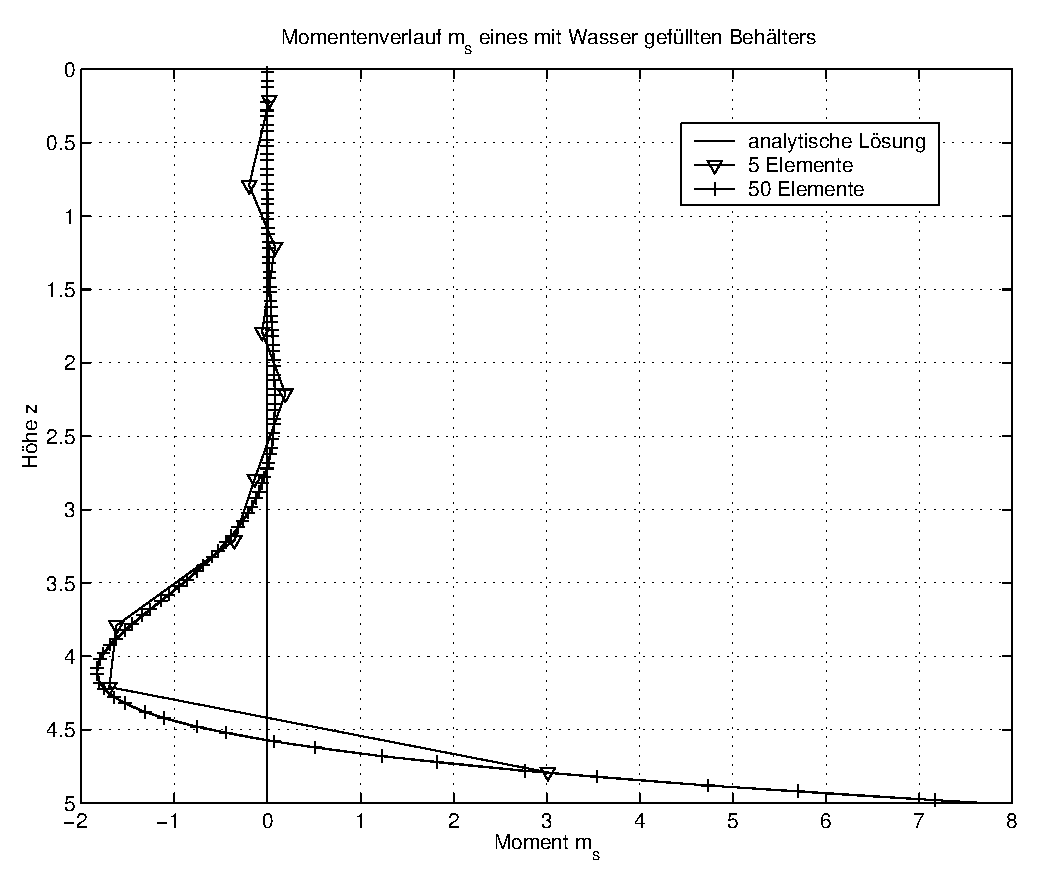
\epsfig{file=\dir/zyl.eps, width=.5\hsize}
\setlength{\baselineskip}{11pt}
\caption{Distribution of stress resultant $m_s$ over the 
height.}
\label{zyl}
\end{center}
\end{Figure}%

\clearpage
\newpage
{\small
\begin{verbatim}
      subroutine elmt05(d,ul,xl,ix,tl,s,p,ndf,ndm,nst,isw)
c-----------------------------------------------------------------------
c     elmt05  : Main-subroutine for a rotation-symmetric shell element
c               with rotation-symmetric loading
c
c     Parameter list
c       d(1-3)       Material- and element parameter
c       d(1) = yo    - Modulus of elasticity
c       d(2) = nu    - Poisson's number
c       d(3) = thick - Shell thickness 
c       d(4)         Number of Gauss-points
c       ul(ndf,*)    Solution vector
c       xl(ndm,nel)  Coordinates of nodes
c       ix(nel)      Global node number
c       tl(nst)      Temperature values of nodes
c       s(nst,nst)   Stiffness matrix
c       p(nst)       Load vector, residuum
c       ndf          Number of degrees of freedom
c       ndm          Dimension of nodes
c       nst          Number of degress of freedom of elements
c       isw          Execution flag
c-----------------------------------------------------------------------
      implicit none
      include   'bdata.h'
      include   'cdata.h'
      include   'debugs.h'
      include   'eldata.h'
      include   'iofile.h'
      integer ix(*)
      integer ndf,ndm,nst,isw
      integer nod,ll,i,j,kk,l
      real*8 d(*),ul(ndf,*),xl(ndm,*),tl(*),s(nst,nst),p(*)
      real*8 aa(4,4),bmat(4,nst),btc(nst,4)
      real*8 sg(5),wg(5)
      real*8 eps(4),sig(4),vl(6),help(6,1),coor(2)
      real*8 yo,nu,thick,sn,cs,sl,rr,Pi,dvol
      logical errck,pinput
c
      if(isw.eq.1) then
c-----------------------------------------------------------------------
c...  Input of material values
    1 if(ior.lt.0) write(*,3000)
        errck=pinput(d,4)
        if(errck) go to 1
        if(ior.lt.0) then
          write(*,2000) d(1),d(2),d(3),d(4)
        end if
        write(iow,2000) d(1),d(2),d(3),d(4)
c
      elseif(isw.eq.2) then
c-----------------------------------------------------------------------
c...  Element check for mistakes
        if(d(3) .le. 0.d0) then
          write(*,*)'  shell_thickness .le. 0'
          stop
        endif
c 
      elseif(isw.eq.3 .or. isw.eq.4) then
c-----------------------------------------------------------------------
c...  Calculation of the stiffness matrix and the residuum 
c...  Material- and element parameter
        yo    = d(1)
        nu    = d(2)
        thick = d(3)
        Pi = 4.d0*datan(1.d0)
c...  Length and angle
        sn = xl(2,2) - xl(2,1)
        cs = xl(1,2) - xl(1,1)
        sl = dsqrt(cs*cs + sn*sn)
        sn = sn/sl
        cs = cs/sl
c...  Calculation of the local displacements
        call pzero(vl,6*1)
        vl(1) =       cs*ul(1,1) + sn*ul(2,1)
        vl(2) = -1.d0*sn*ul(1,1) + cs*ul(2,1)
        vl(3) = ul(3,1)
        vl(4) =       cs*ul(1,2) + sn*ul(2,2)
        vl(5) = -1.d0*sn*ul(1,2) + cs*ul(2,2)
        vl(6) = ul(3,2)
c...  Elasticity matrix and in advance integration
        call pzero(aa,4*4)
        call dmat05(yo,nu,thick,aa)
c...  Labeling of the output list
        if (isw.eq.4) then
           write(iow,100)
           write(iow,101)
        end if
c...  Number of Gauss-points and calculation of the sampling points
        ll = idint(d(4))
        call gauss05(ll,sg,wg)
c.... Gauss loop
        do l = 1,ll
          rr = (1.d0 - sg(l))*xl(2,1) + sg(l)*xl(2,2)
          dvol = rr*2.d0*Pi*sl*wg(l)
          call pzero(bmat,4*nst)
          call bmat05(bmat,sg(l),sl,sn,cs,rr)
c...  Calculation of the strains
          call pzero(eps,4*1)
          do i=1,4
            do j=1,nst
              eps(i) = eps(i) + bmat(i,j)*vl(j)
            end do
          end do
c...  Calculation of the internal force variables
          call pzero(sig,4*1)
          do i=1,4
            do j=1,4
              sig(i) = sig(i) + aa(i,j)*eps(j)
            end do
          end do
          if(isw .eq. 4)then
c.... Display statements, internal force variables into output file
          open(1, file='beisp1.dat')
          coor(1) = xl(1,1) + sl*cs*sg(l)
          coor(2) = xl(2,1) + sl*sn*sg(l)
          write(iow,103) coor(1),coor(2),sig(1),sig(2),sig(3),sig(4)
          write(1,103) coor(1),coor(2),sig(1),sig(2),sig(3),sig(4)

          elseif(isw .eq. 3)then
c...  Calculation of the residuum
          call pzero(help,6*1)
          do i=1,nst
            do j=1,4
              help(i,1) = help(i,1) + bmat(j,i)*sig(j)*dvol
            end do
          end do
          call trans05(help,nst,1,cs,sn,3,2)
          do i=1,nst
            p(i) = p(i) - help(i,1)
          end do
c...  Calculate B^T C
          call pzero(btc,6*4)
          do i  = 1,nst
            do j  = 1,4
               do kk = 1,4
                  btc(i,j) = btc(i,j) + bmat(kk,i)*aa(kk,j)*dvol
               enddo
            enddo
          enddo
c...  Calculate B^T C B = stiffness matrix
          do i  = 1,nst
            do j  = 1,nst
              do kk = 1,4
                s(i,j) = s(i,j) + btc(i,kk)*bmat(kk,j)
              enddo
            enddo
          enddo
        endif    ! end of calculation of the local stiffness matrix
        end do   ! Gauss-loop
c...  Transformation of the stiffness matrix
        if(isw .eq. 3) then
          call trans05(s,nst,nst,cs,sn,ndf,1)
          call trans05(s,nst,nst,cs,sn,ndf,2)
        endif
c
c
      endif   !isw=1,2,3,4,5,6,7,8
c
c----------------------------------------------------------------------
c...  Formate statements
 100  format(15x, 'internal_force_variables')
 101  format(6x,'z',5x,'r',10x,'n_s',8x,'n_theta',8x,'m_s',
     &             8x,'m_theta')
 103  format(5x,f5.2,1x,f5.2,1x,e12.5,1x,e12.5,1x,e12.5,1x,e12.5)
2000  format(5x,'Axis-symmetric shell element:'//
     &   5x,'Modulus of elasticity                yo = ',e12.5/
     &   5x,'Poisson's number                     nu = ',e12.5/
     &   5x,'Shell thickness                       t = ',e12.5/
     &   5x,'Number of Gauss-points               ll = ',I5//)
3000  format(' Input: Yo, nu, t, ll'/'   >',$)
      end
c
c
c
      subroutine gauss05(ll,sg,wg)
c-----------------------------------------------------------------------
c     Sampling points and weighting fo Gauss-point-integration from 0 - 1
c     ll    - Numer of Gauss-points
c     sg(5) - Sampling points
      wg(5) - Weightings
c-----------------------------------------------------------------------
      implicit none
      integer ll
      real*8 sg(5),wg(5)
c
c...  1 Gauss-points
      if(ll .eq. 1) then
        sg(1) = 0.5d0
        wg(1) = 1.d0
c...  2 Gauss-points
      elseif(ll .eq. 2) then
        sg(1) = 0.5d0*(1.d0 - 1.d0/dsqrt(3.d0))
        sg(2) = 0.5d0*(1.d0 + 1.d0/dsqrt(3.d0))
        wg(1) = 0.5d0
        wg(2) = wg(1)
c...  3 Gauss-points
      elseif(ll .eq. 3) then
        sg(1) = 0.5d0*(1.d0 - dsqrt(3.d0/5.d0))
        sg(2) = 0.5d0
        sg(3) = 0.5d0*(1.d0 + dsqrt(3.d0/5.d0))
        wg(1) = 5.d0/18.d0
        wg(2) = 4.d0/9.d0
        wg(3) = wg(1)    
c...  4 Gauss-points
      elseif(ll .eq. 4) then
        sg(1) = 0.5d0*(1.d0 - dsqrt((15.d0 + 2.d0*dsqrt(30.d0))/35.d0))
        sg(2) = 0.5d0*(1.d0 - dsqrt((15.d0 - 2.d0*dsqrt(30.d0))/35.d0))
        sg(3) = 0.5d0*(1.d0 + dsqrt((15.d0 - 2.d0*dsqrt(30.d0))/35.d0))
        sg(4) = 0.5d0*(1.d0 + dsqrt((15.d0 + 2.d0*dsqrt(30.d0))/35.d0))
        wg(1) = .25d0*(1.d0 - dsqrt(30.d0)/18.d0)
        wg(2) = .25d0*(1.d0 + dsqrt(30.d0)/18.d0)
        wg(3) = wg(2)
        wg(4) = wg(1) 
c...  5 Gauss-points
      elseif(ll .eq. 5) then
        sg(1) = 0.5d0*(1.d0 - dsqrt(5.d0 + 4.d0*dsqrt(5.d0/14.d0))/3.d0)
        sg(2) = 0.5d0*(1.d0 - dsqrt(5.d0 - 4.d0*dsqrt(5.d0/14.d0))/3.d0)
        sg(3) = 0.5d0
        sg(4) = 0.5d0*(1.d0 + dsqrt(5.d0 - 4.d0*dsqrt(5.d0/14.d0))/3.d0)
        sg(5) = 0.5d0*(1.d0 + dsqrt(5.d0 + 4.d0*dsqrt(5.d0/14.d0))/3.d0)
        wg(1) = (322.d0 - 13.d0*dsqrt(70.d0))/1800.d0
        wg(2) = (322.d0 + 13.d0*dsqrt(70.d0))/1800.d0
        wg(3) =  64.d0/225.d0
        wg(4) = wg(2)
        wg(5) = wg(1)
      else
        write(*,*)'    Number of Gauss-points is not correct'
        stop
      endif
      return
      end
c
      subroutine bmat05(bmat,xi,sl,sn,cs,rr)
c--------------------------------------------------------------------72
c     Calculation of the B-Operator
c       Paramter list
c       bmat(4,6)  B-Operator
c       xi         Gauss-point
c       sl         Length of element
c       sn         Sinus
c       cs         Cosinus
c       rr         Radius
c----------------------------------------------------------------------
      implicit none
      real*8 bmat(4,6)
      real*8 sl,sn,cs,rr,xi
c
c...  Calculation of the B-Operator
      bmat(1,1) = -1.d0/sl
      bmat(2,1) = (1.d0 - xi)*sn/rr
      bmat(2,2) = (1.d0 -  3.d0*xi*xi + 2.d0*xi*xi*xi)*cs/rr
      bmat(2,3) = (xi - 2.d0*xi*xi + xi*xi*xi)*cs*sl/rr
      bmat(3,2) = -(6.d0 - 12.d0*xi)/(sl*sl)
      bmat(3,3) = -(4.d0 - 6.d0*xi)/sl
      bmat(4,2) = -(6.d0*xi - 6.d0*xi*xi)*sn/(rr*sl)
      bmat(4,3) = -(-1.d0 + 4.d0*xi - 3.d0*xi*xi)*sn/rr
      bmat(1,4) = 1.d0/sl
      bmat(2,4) = xi*sn/rr
      bmat(2,5) = (3.d0*xi*xi - 2.d0*xi*xi*xi)*cs/rr
      bmat(2,6) = (-1.d0*xi*xi + xi*xi*xi)*cs*sl/rr
      bmat(3,5) = -(-6.d0 + 12.d0*xi)/(sl*sl)
      bmat(3,6) = -(2.d0 - 6.d0*xi)/sl
      bmat(4,5) = -(-6.d0*xi + 6.d0*xi*xi)*sn/(rr*sl)
      bmat(4,6) = -(2.d0*xi - 3.d0*xi*xi)*sn/rr
      return
      end
c
      subroutine dmat05(yo,nu,thick,aa)
c---------------------------------------------------------------------72
c     Calculation of the material matrix, 
c     in advance integration over the shell thickness
c     Parameter list
c       yo      Modulus of elasticity
c       nu      Poisson's number 
c       thick   Shell thickness
c       aa(4,4) Material matrix
c----------------------------------------------------------------------
      implicit none
      real*8 yo,nu,thick,fakt
      real*8 aa(4,4)
c
      fakt = yo*thick/(1.d0-nu*nu)
      aa(1,1) = fakt * 1.d0
      aa(1,2) = fakt * nu
      aa(2,1) = aa(1,2)
      aa(2,2) = aa(1,1)
      aa(3,3) = fakt * thick*thick/12.d0 
      aa(3,4) = nu * aa(3,3)
      aa(4,3) = aa(3,4) 
      aa(4,4) = aa(3,3)
c
      return
      end
c
c
      subroutine trans05(a,n,m,cs,sn,k,iswl)
c-----------------------------------------------------------------------
c     Transformation of a matrix
c        a(n,m)      Matrix        
c        n,m         Rows, columns
c        cs          Cosinus
c        sn          Sinus
c        k           Step size of the loop
c        iswl        Control-variable
c-----------------------------------------------------------------------
      implicit none
c
      integer i,j,n,m,k,iswl
      real*8 t,cs,sn
      real*8 a(n,m)
c    
c...  S * T
      if (iswl.eq.1) then
        do i=1,m,k
          do j=1,n
            t        = a(j,i)*cs - a(j,i+1)*sn
            a(j,i+1) = a(j,i)*sn + a(j,i+1)*cs
            a(j,i)   = t
          end do
        end do
c
c...  T^T * S * T
      elseif (iswl.eq.2) then
        do i=1,n,k
          do j=1,m
            t        = a(i,j)*cs - a(i+1,j)*sn
            a(i+1,j) = a(i,j)*sn + a(i+1,j)*cs
            a(i,j)   = t
          end do
        end do
      end if
c
      return
      end
\end{verbatim}
}

 
